\documentclass[12pt, titlepage]{article}
\usepackage[utf8]{inputenc}
\usepackage{float}
\usepackage[ngerman]{babel}
\usepackage[stable]{footmisc}
\usepackage{graphicx}
\usepackage[a4paper,lmargin={2cm},rmargin={2cm},
tmargin={2.5cm},bmargin = {2.5cm}]{geometry}
\usepackage{caption}
\usepackage{tikz}
\newcommand*\annotatedFigureBoxCustom[8]{\draw[#5,thick,rounded corners] (#1) rectangle (#2);\node at (#4) [fill=#6,thick,shape=circle,draw=#7,inner sep=2pt,font=\sffamily,text=#8] {\textbf{#3}};}
\newcommand*\annotatedFigureBox[4]{\annotatedFigureBoxCustom{#1}{#2}{#3}{#4}{lightgray}{white}{black}{black}}
\newcommand*\annotatedFigureText[4]{\node[draw=none, anchor=south west, text=#2, inner sep=0, text width=#3\linewidth,font=\sffamily] at (#1){#4};}
\newenvironment {annotatedFigure}[1]{\centering\begin{tikzpicture}
\node[anchor=south west,inner sep=0] (image) at (0,0) { #1};\begin{scope}[x={(image.south east)},y={(image.north west)}]}{\end{scope}\end{tikzpicture}}

\usepackage{adjustbox}
\let\oldhash\#%
\DeclareRobustCommand{\#}{\adjustbox{valign=B,totalheight=.57\baselineskip}{\oldhash}}%

\usepackage{hyperref}
\hypersetup{
    colorlinks,
    citecolor=black,
    filecolor=black,
    linkcolor=black,
    urlcolor=blue
}

\usepackage{color}
\definecolor{codegreen}{rgb}{0,0.6,0}
\definecolor{codegray}{rgb}{0.5,0.5,0.5}
\definecolor{codepurple}{rgb}{0.58,0,0.82}
\definecolor{backcolour}{rgb}{0.95,0.95,0.92}

\usepackage{listings}
\lstset{literate=%
  {Ö}{{\"O}}1
  {Ä}{{\"A}}1
  {Ü}{{\"U}}1
  {ß}{{\ss}}1
  {ü}{{\"u}}1
  {ä}{{\"a}}1
  {ö}{{\"o}}1
}
\lstdefinestyle{code}{
    backgroundcolor=\color{backcolour},   
    commentstyle=\color{codegreen},
    keywordstyle=\color{magenta},
    numberstyle=\tiny\color{codegray},
    stringstyle=\color{codepurple},
    basicstyle=\ttfamily\footnotesize,
    breakatwhitespace=false,         
    breaklines=true,
    lineskip=2pt,                
    captionpos=b,                    
    keepspaces=true,
    language=[Sharp]C,
    morekeywords={int2},
    numbers=left,                    
    numbersep=5pt,                  
    showspaces=false,                
    showstringspaces=false,
    showtabs=false,                  
    tabsize=2,
    inputencoding=utf8,
    moredelim=**[is][\color{blue}]{~}{~},
    moredelim=**[is][\color{red}]{@}{@},
}

\linespread{1.25}

%Variablen
\newcommand{\myTitle}{Steigerung der Performance in Videospielen durch datenorientierte Programmierung}

\begin{document}
\begin{titlepage}
\centering
{\huge Friedrich-Schiller-Universität Jena \par}
{\large Fakultät für Mathematik und Informatik\par}
\vspace{1.5cm}
{\huge\bfseries \myTitle\par}
\vspace{2cm}
{\Large Bachelorarbeit zur Erlangung des akademischen Grades\\Bachelor of Science (B.Sc.) \par}
\vspace{3cm}
{\large vorgelegt von Dennis Untiet\\Matrikelnummer: 192151\par}
\vspace{0.5cm}
{\large geboren am 01.10.2001\quad in Esslingen\par}
\vspace{2cm}
{\large Erstgutachter: Joachim Giesen \\Zweitgutachter: Julien Klaus\par} 
\vfill
{\Large Jena, \today}
\end{titlepage}
\newpage 
\thispagestyle{empty}
\quad
\newpage
\thispagestyle{empty}
\section*{Zusammenfassung}
Die vorliegende Arbeit befasst sich mit der Performancesteigerung in Videospielen durch Datenorientierte Programmierung. Mit dem datenorientierten Ansatz wird versucht, die objektorientierte, nicht Cache freundliche Verarbeitung von Daten zu ersetzen. Der Fokus wird auf die Art und Weise gelegt, wie Daten im Speicher liegen, gelesen, geschrieben und verarbeitet werden. Hierdurch soll eine schnellere Verarbeitung der Daten erreicht werden. Eine mögliche Implementierung ist dabei der \textit{Datenorientierte Technologie-Stack} von Unity. In dieser Arbeit wird die Leistungssteigerung betrachtet, die ein datenorientierter Ansatz bietet. Dazu wurde eine Spielesimulation in Unity einmal objektorientiert und einmal datenorientiert entwickelt, welche anschließend gebenchmarkt wurde. Die Umsetzung des datenorientierten Spiels gestaltete sich schwieriger, als die des objektorientierten Spiels. Die Benchmarks ergaben, dass durch einen datenorientierten Ansatz eine enorme Performancesteigerung möglich ist.
\newpage
\thispagestyle{empty}
\quad
\newpage
\tableofcontents
\newpage 
\thispagestyle{empty}
\quad
\newpage
\section{Einleitung}
Die Videospielbranche ist eine der größten Marktzweige die es auf der Welt gibt. Laut dem Marktforschungsunternehmen Newzoo hatte die Gaming-Industrie 2021 einen Gesamtumsatz von rund 192,7 Milliarden Dollar weltweit \cite{Spiele-Industrie-weltweit}. Dies ist mehr Umsatz, als Filme-, Serien- und aufgenommene Musikindustrie zusammengenommen. Auch in Deutschland liegt der Umsatz der Gaming-Industrie knapp vor dem Umsatz des Videostreamings und der Musik \cite{Spiele-Industrie-deutschland}.\\
Die Videospiele, welche heutzutage auf den Markt kommen, werden immer komplexer. Es werden immer größere Spiele entwickelt, welche mit immer mehr Inhalt gefüllt werden. Diese müssen aber natürlich trotzdem, oder vielleicht gerade deshalb auch Leistungsstandards entsprechen. Um diesen Anforderungen gerecht zu werden, sind fortschrittliche Programmieransätze erforderlich, die die Performance-Steigerung in komplexen Videospielen ermöglichen. Zwar steigt die Rechenleistung in modernen Computern weiter an, es passiert aber dennoch immer wieder, dass Spiele mit einem Objektorientierten Ansatz an ihre Grenzen stoßen, die Rechenleistung vollständig umzusetzen. Auch ist es sinnvoll, Videospiele energieeffizienter zu gestalten um Stromeinsparungen und Nachhaltigkeit zu erhalten. Das heißt, es wird in Zukunft wesentlich wichtiger sein, einen alternativen Lösungsansatz anzustreben, statt die immer größer werdende Rechenleistung auszunutzen. Dabei können ein Datenorientierter Ansatz bei der Programmierung und Parallelisierung des Programms eine Lösung sein.\\
Die vorliegende Arbeit geht dabei insbesondere auf den Datenorientierten Ansatz von Unity, also das \textit{Entity Component System} (ECS), ein. Die Spiele-Engine Unity wurde aus den folgenden Gründen gewählt:\\
1. Unity ist eine Spiele-Engine, welche führend in der Spiele-Industrie ist. Mit ihr wurden schon viele große Spiele entwickelt\footnote{https://www.thegamer.com/unity-game-engine-great-games/}.\\
2. Das ECS von Unity befindet sich momentan in großer Entwicklung. Unity setzt viel daran, den Datenorientierten Technologie-Stack auszubauen und es kamen viele Neuerungen in den letzten Monaten\footnote{https://unity.com/de/roadmap/unity-platform/dots}.
\newpage
\section{datenorientierte Programmierung}
\subsection{Was ist das datenorientierte Design?}
Data-Oriented Design \cite{Data-OrientedDesign}\\
Probleme mit OOP: Hauptspeicher Zugriff und Cache misses. Versuche Code zu Parallelisieren sind zu viel Aufwand und bringen kaum etwas. Code ist sehr komplex.\\Datenorientiertes Design ist ein anderer Ansatz, der diese Probleme zu lösen versucht. Datenorientierung ändert die Sichtweise des Programmierens: Weg von Objekten, hin zu den eigentlichen Daten, wie diese im Speicher liegen und wie sie gelesen und verändert werden. Beim Programmieren geht es immer um das Verändern von Daten. Es ist die Beschreibung wie aus eingegebenen Daten veränderte Daten werden. Daher ergibt es Sinn sich direkt mit den Daten zu befassen. Zusätzlich: \glqq data-oriented design\grqq{}  hat nichts mit \glqq data-driven\grqq{} zu tun.\\ Ideale Daten:\\Kommt auf die Daten an und wie sie genutzt werden. Am besten wenn man die Daten mit möglichst geringem Aufwand nutzen kann. Also kleinstmögliche Veränderung. Das Programms wird um die ideale Datenstruktur gebaut.\\Objekte sind oft wie Bäume gebaut. Objekte interagieren oft mit anderen Objekte \glqq unter\grqq{} ihnen. Iteriert man über eine Anzahl an Objekten passiert das mehrfach mit beliebigen Objekten. Für ein Ideales Layout sollte ein Objekt in Komponenten zerlegt werden. Komponenten der gleichen Art können dann als Gruppe zusammen im Speicher liegen, egal von welchem Objekt sie kommen. Daraus resultierten große Gruppe homogener Daten, welche dann sequenziell verarbeitet werden können.\\Vorteile:\\Parallelisierung: Die Daten können sehr leicht auf mehrere Threads aufgeteilt werden ohne großen Aufwand\\Cache Affinität: Sehr Effizient, da der selbe Code immer wieder ausgeführt wird. Wenn die Daten sequenziell verarbeitet werden resultiert das in sehr guter Performance und fast perfekter Cache Nutzung.\\Modularität: Wenn Code zur Verbesserung der Performance angepasst wird, resultiert das oft in schlechter lesbarem und schlechter wartbarem Code. Bei Konzentration auf die Transformierung der Daten hat man am Ende kleinere Funktionen mit weniger Abhängigkeiten.\\Testing: Unit Test für Objektinteraktionen können kompliziert sein. Im Datenorientierten Design sind Unit Tests jedoch sehr einfach. Eingabe Daten erstellen, Funktion aufrufen und die Ausgabedaten verifizieren.\\Nachteile: Nicht die Lösung für alles. Schwierig zu lernen, da es ganz anders ist. Auch schwierig mit bestehendem prozedurale / Objektorientiertem Code zu verbinden.\\Anwendung: Klassifizierung, wie Daten genutzt werden: read-only / read-write / write-only. Welche Daten werden von dem System gebraucht? Nicht wie verhält sich ein Gegner sonder eher wie sich alle verhalten.\\Platz für OOP?: Teils / teils. Für einzelne Objekte (beispielsweise GUI) kann es sinnvoll sein. Sollte aber dennoch Datenorientiert geschrieben werden.
\\ DOD \cite{DOD}\\
Datenorientiertes Design kann auch mit anderen Programmier Paradigmen co-existieren. Datenorientierung wird mehr gebraucht, da Spiele immer komplexer werden und die Abstraktion durch OOP das Bottleneck sein wird. Überall sind Daten: Graphik auf dem Bildschirm, Positionen und Bewegung von Partikeln und so weiter. All diese Daten müssen auf etwas laufen, sei es eine VM oder etwas konkretes wie der CPU oder der GPU. Diese Daten existieren auf der Hardware irgendwo. Datenorientiertes Design ist das designen von Software, welche Transformationen auf wohldefinierten Daten ausführt. \\
Ein einfaches Beispiel:\\Angenommen man hat im Objektorientierten Personen Objekte, welche Attribute haben, wie Alter, Beruf und Geschlecht. Dann würden diese Daten im datenorientierten beispielsweise in einer Liste gespeichert werden. Wenn man jetzt das Durchschnittsalter von allen vorhandenen Personen errechnen will muss man im Objektorientierten alle Objekte einzeln ansprechen und dort das Alter abfragen und diese dann verrechnen. Im datenorientierten kann man sich aber direkt die Liste von allen Personen hernehmen. Somit ist der Zugriff und die Berechnung des Durchschnittsalter wesentlicher schneller.
\subsection{Umsetzung Datenorientierter Programmierung}
\newpage
\section{Unity's Datenorientierter Technologie-Stack\footnote{https://unity.com/de/dots}}
Die Arbeit basiert auf der Entities Version 1.0.0-pre.65. Dies ist Stand dem 01.04.2023 die aktuellste Version von Unity's \textit{Enitity Component System.}. Da die Version noch nicht final fertiggestellt wurde und noch stark bei Unity in Arbeit ist, kann sich mit der Zeit viel an der Art und Weise, wie Unity Datenorientierte Programmierung umsetzt, ändern. Das Grundkonzept der Datenorientierung Programmierung ist allerdings mit dem Datenorientierten Technologie-Stack festgeschrieben.\\
Unity's Datenorientierter Ansatz wird durch Unity's Datenorientierter Technologie-Stack umgesetzt. Dieser besteht aus drei Teilen:\\
1. Das \textit{Entity Component System} (ECS) für Unity. Dies ist ein Daten-orientierter Framework für Unity. Dieser ist auch kompatibel mit GameObjects, was Unity's üblicher Objektorientierter Ansatz ist.\\
3. Das C\# Job System. Das Job System von Unity erlaubt es parallelen Code zu schreiben, welcher sicher und schnell läuft.\\
2. Der \textit{Burst Compiler}. Der Burst Compiler übersetzt von IL/.NET Bytecode zu optimierten nativen Code. Es nutzt die LLVM Compiler Infrastruktur.\\
Diese drei Teile werden in den folgenden Katpiteln \ref{ecs}, \ref{burst} und \ref{jobs} erklärt
\subsection{Objektorientierte Programmierung in Unity}
Bevor das \textit{Entity Component System} betrachtet wird ein kleiner Exkurs zu der herkömmlichen Weise, wie in Unity gearbeitet wird. Dies ist hilfreich um folgende Kapitel besser zu verstehen. In Unity basiert alles auf \textit{GameObjects}, die das Objektorientierte schon im Namen haben. Die \textit{GameObjects} werden immer in einer Szene erstellt, wobei es mehrere Szenen in einem Projekt geben kann. Es kann beispielsweise eine Szene für den Startbildschirm geben und eine Szene für das eigentliche Spiel. Alles was man in seiner Szene erstellt ist zunächst ein \textit{GameObject} welches man dann mit Leben füllt. Durch Komponenten die man dem \textit{GameObject} gibt, kann man sie zu Licht, Charakteren, oder Gegenständen werden lassen. Die Komponenten sind allerdings anders als die \textit{Components} aus dem \textit{Entity Component System}. In den folgenden Abschnitten erkennt man hierbei jedoch viele Parallelen zu dieser Arbeitsweise. Die Art wie man Code schreibt ist jedoch sehr unterschiedlich. Zugriffe auf Daten anderer \textit{GameObjects} funktionieren so, dass man erst auf das \textit{GameObject} zugreift und dann darüber auf seine Komponenten. Also ein typische Objektorientierter Ansatz.
\subsection{Das \textit{Entity Component System}} \label{ecs}
\begin{figure}[H]
\begin{center}
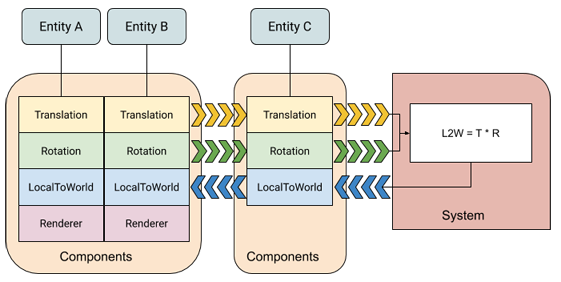
\includegraphics[scale=0.8]{Bilder/ECSConcept.png}
\caption{Zusammenspiel von \textit{Entities}, \textit{Components} und Systemen. Beispielhaft werden hier 3 \textit{Entities} gezeigt, wobei \textit{Entity} A und B fünf \textit{Components} haben und \textit{Entity} C nur vier \textit{Components} hat. \textit{Entity} C fehlt also das \texttt{Renderer} \textit{Component}. Das System nimmt als Eingabe alle \texttt{Translation} und \texttt{Rotation} \textit{Components} und modifiziert damit das \texttt{LocalToWorld} \textit{Component} der \textit{Entities}.}
\label{fig:ecs_concept}
\end{center}
\end{figure}
\subsubsection{\textit{Entities}\footnote{https://docs.unity3d.com/Packages/com.unity.entities@1.0/manual/concepts-entities.html}}\textit{Entities} repräsentieren meist Dinge in einem Unity Spiel. Das kann der Spielcharakter, Gegenstände, oder beliebige Gegner sein. Sie können aber auch abstrakte Dinge, wie beispielsweise Events repräsentieren. Ein Entity ist vergleichbar mit einem \textit{GameObject} im Objektorientierten in Unity. \textit{Entities} besitzen hierbei jedoch weder Daten noch ein Verhalten, sondern zeigen lediglich auf, welche Daten beziehungsweise \textit{Components} zueinander gehören. Alle \textit{Entities} in einer Spielwelt gehören zu einer sogenannten Welt\footnote{https://docs.unity3d.com/Packages/com.unity.entities@0.1/manual/world.html}. Zu dieser Welt gehört genau ein \textit{Entitymanager}\footnote{https://docs.unity3d.com/Packages/com.unity.entities@1.0/api/Unity.Entities.EntityManager.html}. Der \textit{Entitymanager} organisiert alle \textit{Entities} in dieser Welt. Mit ihm lassen sich \textit{Entities} erstellen, zerstören, \textit{Components} zu \textit{Entities} hinzufügen, entfernen oder verändern.
\subsubsection{\textit{Components}\footnote{https://docs.unity3d.com/Packages/com.unity.entities@1.0/manual/concepts-components.html}}
\textit{Components} repräsentieren die Daten des Spiels. \textit{Components} speichern die Daten eines \textit{Entity}. Diese Daten werden von Systemen genutzt und verarbeitet. Dabei unterscheidet man zwischen verwalteten \textit{Components} und unverwalteten \textit{Components}. Unverwaltete \textit{Components} werden in Unity als C\# Strukturen implementiert, sind leichtgewichtiger als Klassen. Diese können auch nur unverwaltete Daten speichern. Unverwaltete Daten sind beispielsweise Integer, Boolean, Bytes, Chars, oder andere Strukturen. Verwaltete \textit{Components} werden hingegen als Klassen definiert und können alle Daten halten. Es ist jedoch üblich unverwaltete \textit{Components} zu verwenden, da diese nicht so resourcenintensiv im Speichern und Zugriffen sind. Um ein unverwaltetes Component zu erstellen kann man das IComponentData Interface verwenden. Ein einfaches \textit{Component} könnte also wie folgt aussehen:
\begin{lstlisting}[style=code, caption={Beispiel unverwaltetes \textit{Component}}]
using Unity.Entities;
using Unity.Mathematics;

namespace ECS.Components
{
    public struct ExampleComponent : IComponentData
    {
        public int2 position;
        public float speed;
    }
}
\end{lstlisting}
Es gibt aber auch andere Arten von \textit{Components}. Es gibt \textit{Shared components}, \textit{Buffer components} und weitere\footnote{https://docs.unity3d.com/Packages/com.unity.entities@1.0/manual/components-type.html}. Es sind hier nicht alle \textit{Components} relevant, da manche lediglich die Spieleentwickelung mit dem datenorientierten Ansatz erleichtern, aber keine neue Funktion bieten. Zudem gibt es alle Arten von \textit{Components} sowohl als verwaltete als auch unverwaltete \textit{Components}.\\
\textbf{\textit{Shared Components}}: \textit{Shared Components} sind wie der Name schon sagt unter den \textit{Entities} gleich. Sie gruppieren die \textit{Entities} nach dem Wert des \textit{Shared Component}. \textit{Shared Components} werden abseits anderer \textit{Components} gespeichert und sind ein Weg um Datenduplizierung zu vermeiden. Unity speichert zusätzlich alle \textit{Entities}, welche die gleiche Kombination aus \textit{Component} Typen haben und das gleiche \textit{Shared Component} haben, also auch den gleichen Wert, gemeinsam. Dies hat zwar Vorteile, aber auch den großen Nachteil, dass das Ändern von Werten des \textit{Shared Component} ein verschieben der \textit{Entities} im Speicher zufolge hat. Die Probleme hierbei findet man in Kapitel \ref{structuralChanges}. Einen sehr großen und sinnvollen Vorteil haben \textit{Shared Components} in jedem Spiel das mit Unity's ECS entwickelt wird. Das RenderMesh \textit{Component}, also das \textit{Component} welches für das Aussehen der \textit{Entities} zuständig ist, ist immer ein \textit{Shared Component}. Dies ist sinnvoll, da sich diese \textit{Component} sehr selten im Wert ändert und viele \textit{Entities} das selbe RenderMesh \textit{Component} besitzen. Das kann ganz simpel einfach das Aussehen eines Baumes in einem Spiel sein. Oft gibt es viele Bäume in dem Spiel und diese ändern auch ihr Aussehen nicht.\\
\textbf{\textit{Buffer Components}}: Falls man mehrere \textit{Components} der selben Art auf einem \textit{Entity} haben möchte, sind \textit{Buffer Components} sehr hilfreich. Diese agieren wie ein Array von \textit{Components}. Zusätzlich sind \textit{Buffer Components} der Weg um ein Array an Daten zu speichern. Das ist besonder hilfreich, wenn man einem \textit{Entity} ein Inventar geben möchte, da dieses aus mehreren Gegenständen bestehen kann. Also kann man beispielsweise ein \textit{Buffer Component} für ein Inventar so entwerfen:
\begin{lstlisting}[style=code, caption={Buffer \textit{Component} Beispiel}]
using Unity.Entities;

namespace ECS.Components.Other
{
	//Array Kapazität auf acht festlegen
    [InternalBufferCapacity(8)]
    public struct ItemAmount : IBufferElementData
    {
        public int itemID;
        public int amount;
    }
}
\end{lstlisting}
Wie man sieht leitet die Struktur diesmal von IBufferElementData ab, welche den Typ \textit{Buffer Component} angibt. Zusätzlich wird hier das Attribut \textit{InternalBufferCapacity} genutzt. Damit legt man die Kapazität des \textit{Components} fest. Standardmäßig ist die Kapazität die Anzahl an Elementen, welche in 128 Bytes passen. Also hätten wir bei diesem Beispiel eine Kapazität von 16, da in einem \textit{Component} zwei Integer à 32 bit gespeichert werden. Jedoch braucht man für das Inventar beispielsweise nur 8 zu speichernde Gegenstände und kann so den benötigten Speicherplatz reduzieren.
\subsubsection{Systeme\footnote{https://docs.unity3d.com/Packages/com.unity.entities@1.0/manual/concepts-systems.html}}
Systeme beschreiben das Verhalten und beinhalten die Logik zum Transformieren der Daten. Die Systeme laufen ein mal pro ausgegebenem Bild mithilfe der \texttt{OnUpdate} Funktion auf dem \textit{main} Thread. Genau wie bei dem Objektorientierten von Unity gibt es auch hier mehrere Funktionen die zum Start / Ende ausgeführt werden. Zusätzlich kann man noch unter den definierten Systemen eine Reihenfolge festlegen, in der diese ausgeführt werden sollen. So wie bei den \textit{Components} gibt es auch bei den Systemen eine Klasse für verwaltete Daten (welche in diesem Fall von der Klasse SystemBase erbt) und eine Struktur für unverwaltete Daten (welche in diesem Fall das Interface ISystem implementiert). Zusätzlich sind Systeme immer an eine \textit{World} gebunden. Ein System für unverwaltete Daten und ohne implementierte Logik kann folgende Methoden implementieren:
\begin{lstlisting}[style=code, caption={System Beispiel}]
using Unity.Entities;

namespace ECS.Systems
{
    public partial struct ExampleSystem : ISystem, ISystemStartStop
    {
        //Wird beim Erstellen des Systems ausgeführt
        public void OnCreate(ref SystemState state){}
        //Wird vor dem ersten OnUpdate des Systems ausgeführt
        public void OnStartRunning(ref SystemState state){}
        //Wird für jedes ausgegebene Bild ausgeführt
        public void OnUpdate(ref SystemState state){}
        //Wird beim Stoppen des Systems ausgeführt
        public void OnStopRunning(ref SystemState state){}
        //Wird beim Zerstören des Systems ausgeführt
        public void OnDestroy(ref SystemState state){}
    }
}
\end{lstlisting}
Dabei ist das Interface ISystemStartStop optional und bietet die Möglichkeit bei dem Starten und Stoppen des Systems zusätzlich spezielle Logik auszuführen. Wie man sieht wird allen Funktionen auch eine Referenz des \textit{SystemState} übergeben. Darüber kann man auf verschiedene nützliche Dinge zugreifen, wie beispielsweise die \textit{World}, den \textit{EntityManager}, oder aber auch alle \textit{Components} eines Typs. Eine sinnvolle Herangehensweise ist es, in der \texttt{OnUpdate} Funktion Jobs zu schedulen. Dies wird in Kapitel \ref{jobs} weiter beschrieben.
\subsubsection{Archetypen\footnote{https://docs.unity3d.com/Packages/com.unity.entities@1.0/manual/concepts-archetypes.html}}
\begin{figure}[H]
\begin{center}
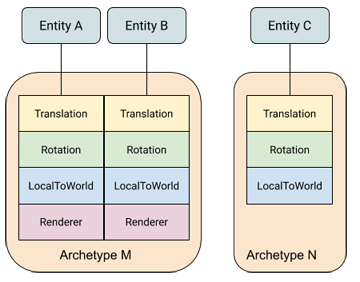
\includegraphics[scale=0.7]{Bilder/ArchetypeConcept.png}
\caption{Konzept von Archetypen. \textit{Entities}, welche die gleiche Zusammenstellung von \textit{Components} haben gehören einem Archetyp an. \textit{Entity} A und B gehören durch die gleiche Zusammenstellung an \textit{Components} also dem Archetyp M an und \textit{Entity} C hat eine andere Zusammenstellung Archetyp N an.}
\label{fig:archetype_concept}
\end{center}
\end{figure}
Ein Archetyp ist eine gewisse Zusammenstellung aus \textit{Components}. Jedes \textit{Entity} kann somit einem Archetyp zugeordnet werden. Beispielsweise sind alle \textit{Entities}, welche nur das ExampleComponent haben, einem Archetyp zugeordnet. \textit{Entities} welche zusätzlich \textit{Component} A besitzen gehören zu einem anderen Archetyp. Durch Archetypen ist es möglich, sehr performant, Datenorientiert zu arbeiten. Möchte man in einem System auf verschiedene \textit{Components} Operationen auszuführen, kann man alle Archetypen nach diesen \textit{Components} druchsuchen und muss nicht alle \textit{Entities} durchsuchen. Zusätzlich kann man diese Anfragen an Archetypen cachen um noch mehr Performance zu erreichen. Unity speichert alle \textit{Components} von \textit{Entities} für ein gewissen Archetyp in einem Block. Dieser wird auch \textit{Chunks} genannt. In Abbildung \ref{fig:archetyp_chunks} sieht man eine Visualisierung wie Archetypen mit \textit{Chunks} zusammenhängen:
\begin{figure}[H]
\begin{center}
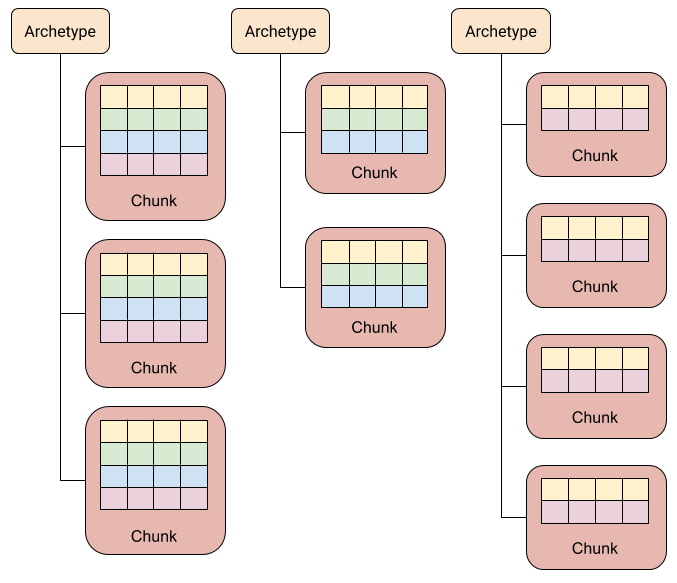
\includegraphics[scale=0.45]{Bilder/ArchetypeChunkDiagram.png}
\caption{Konzept von \textit{Chunks}. \textit{Chunks} sind Speicherbereiche für Archetypen. In dem Bild ist zu erkennen, dass der Archetyp links vier \textit{Components} hat (Anzahl an Reihen), der Archetyp in der Mitte drei \textit{Components} und der Archetyp rechts zwei \textit{Components}. In einen \textit{Chunk} passen hier jeweils vier \textit{Entities}, wobei dies von der Anzahl und Größe der jeweiligen \textit{Components} abhängig ist. Wenn ein \textit{Chunk} voll ist, muss ein neuer \textit{Chunk} erstellt werden. Daher kann es, abhängig von der Anzahl der \textit{Entities} in einem \textit{Chunk}, unterschiedlich viele \textit{Chunks} pro Archetyp geben.}
\label{fig:archetyp_chunks}
\end{center}
\end{figure}
Jeder dieser \textit{Chunks} ist 16 KiB groß. Demnach hängt es von den \textit{Components} ab, wie viele \textit{Entities} in einen \textit{Chunk} passen. Der \textit{Chunk} beinhaltet ein Array für jeden Typ der \textit{Components} und zusätzlich ein Array für die \textit{Entity} ID. Pro Arrayindex wird je ein \textit{Entity} gespeichert. Im Index 0 aller Arrays werden die Daten des ersten \textit{Entities} gespeichert. Falls ein \textit{Entity} zerstört, oder in einen anderen \textit{Chunk} bewegt wird (falls ein \textit{Component} hinzugefügt, oder entfernt wird), wird das letzte \textit{Entity} an seine Stelle bewegt. Falls ein \textit{Chunk} voll ist, erstellt der \textit{EntityManager} einen neuen falls eine \textit{Entity} hinzukommt. Leere \textit{Chunks} werden gelöscht.
\subsubsection{Strukturelle Änderungen}\label{structuralChanges}
Strukturelle Änderungen sind eines der wenigen unperformantem Themen in Unity's \textit{ECS}. Strukturelle Änderungen können das Erstellen und Zerstören eines \textit{Entities}, das Hinzufügen und Entfernen von \textit{Components}, oder das Ändern von Daten eines \textit{Shared Components} sein\footnote{https://docs.unity3d.com/Packages/com.unity.entities@1.0/manual/concepts-structural-changes.html}. Also im Grunde alles Operationen, welches das Ändern eines, oder mehrerer \textit{chunks} erfordert. Solche Änderungen könnten andere zur selben Zeit ausgeführten Aktionen invalidieren und müssen deshalb auf dem main Thread ausgeführt werden. Um dennoch Änderungen dynamisch an beliebiger Stelle ausführen zu können, nutzt man den \textit{Entity Command Buffer} (ECB). Mit dem ECB lassen sich strukturelle Änderungen sammeln und zu einem späteren Zeitpunkt in einer festgelegt Reihenfolge ausführen. So lassen sich problemlos aus einem Job strukturelle Änderungen sammeln und nach Beendigung des Jobs, diese auf dem main Thread ausführen. Das kann beispielsweise so aussehen:
\begin{lstlisting}[style=code, caption={ECB Beispiel}]
public void OnUpdate(ref SystemState state)
{
    //Neuer ECB wird erstellt
    EntityCommandBuffer ecb = new EntityCommandBuffer(Allocator.TempJob);
    //Job wird erstellt und der ECB wird übergeben
    new ExampleJob
    {
        ecb = ecb
    //Mit Schedule wird der Job gestartet
    }.Schedule();
    state.CompleteDependency();
    //Strukturelle Änderungen werden abgespielt
    ecb.Playback(state.EntityManager);
    //ECB muss auch wieder disposed werden
    ecb.Dispose();
}
\end{lstlisting}
Also erstellt man einen ECB, reiht verschiedene Aktionen in die Schlange ein und spielt diese auf dem main Thread wieder ab. Danach sollte man den ECB wieder disposen. Das gibt den Speicher für das Objekt wieder frei und räumt gegebenenfalls weitere Ressourcen auf. In dem Job kann man mit dem übergebenen ECB verschiedene Aktionen durchführen. Dies kann beispielsweise so aussehen:
\begin{lstlisting}[style=code, caption={ECB Aktionen Beispiel}]
//Ein Entity erstellen:
Entity newEntity = ecb.Instantiate(e);
//Dem Entity ein Component hinzufügen:
ecb.AddComponent<ExampleComponent>(newEntity);
\end{lstlisting}
Wie ein Job genau aussieht und funktioniert wird in Kapitel \ref{jobs} beschrieben.
\subsection{Job System} \label{jobs}
Unity's Job System ist ein guter Weg um parallelen Code zu schreiben. Jobs werden meist in der \texttt{OnUpdate} Funktion erzeugt und ausgeführt. Dabei kann man entscheiden ob der Job auf dem \texttt{main} Thread, einem \textit{Worker} Thread, oder mehreren \textit{Worker} Threads ausgeführt werden soll. Die Anzahl an verfügbaren \textit{Worker} Threads wird dabei von der Anzahl an verfügbaren Kernen im Prozessor bestimmt. Nachdem der Job erstellt wurde, kann man ihn mit dem Funktionsaufruf \texttt{Run} (Ausführung auf dem \texttt{main} Thread), \texttt{Schedule} (Ausführung auf einem \textit{Worker} Thread), oder \texttt{ScheduleParallel} (Ausführung auf mehreren \textit{Worker} Threads) ausführen. Zusätzlich gibt es noch verschiedene Jobarten, welche auf die Arbeit mit dem ECS angepasst wurden. Dabei gibt es den \texttt{IJobEntity} und den \texttt{IJobChunk} Job.
\subsubsection{IJobEntity}
Der IJobEntity Job ist der Standard Job um über Daten von \textit{Components} zu iterieren. Mit ihm lässt sich leicht definieren, welche Daten man lesen oder schreiben möchte. Zusätzlich kann man noch weiter Attribute, der in dem Job befindlichen \texttt{Execute} Funktion, übergeben lassen. Ein Beispiel für ein fertig implementierten IJobEntity Job kann wiefolgt aussehen:
\begin{lstlisting}[style=code, caption={IJobEntity Beispiel}, label=IJobEntity]
//Beispiel Component
public struct ExampleComponent : IComponentData { public float Value; }
//Entities mit dem DontWantComponent werden ausgeschlossen
[WithNone(typeof(DontWantComponent))]
//Job ist eine Struktur und implementiert das IJobEntity Interface
public partial struct ExampleJob : IJobEntity
{
	//Execute Funktion wird für jedes ExampleComponent ausgeführt
    void Execute(Entity e, ref ExampleComponent component)
    {
    		//Addiert eins zu jedem ExampleComponent Wert.
        component.Value += 1f;
    }
}
//Beispiel System welches den Job verwendet
public partial class ExampleSystem : ISystem
{
    protected override void OnUpdate()
    {
        //Job wird erstellt und auf mehreren Worker Threads ausgeführt
        new ExampleJob().ScheduleParallel();
    }
}
\end{lstlisting}
Wie man in dem Beispiel sieht ist der Job auch wieder eine Struktur und implementiert das IJobEntity Interface. Durch dieses Interface kann man eine eigene \texttt{Execute} Funktion erstellen und anpassen. Je nach dem, welche \textit{Components} man der \texttt{Execute} Funktion übergibt, werden alle \textit{Entities} die alle diese  \textit{Components} besitzen, an die Funktion mit ihren \textit{Components} übergeben. Falls man die \textit{Entities} weiter einschränken, oder lockern will, welche der Funktion übergeben werden, kann man dies mit den Attributen \texttt{WithNone(typeof(ComponentX))} (\textit{Entities} mit dem ComponentX werden ausgeschlossen), \texttt{WithAll(typeof(ComponentX))} (\textit{Entities} müssen das ComponentX besitzen), oder \texttt{WithAny(typeof(ComponentX), typeof(ComponentY))} (\textit{Entities} müssen das ComponentX, oder das ComponentY besitzen) über dem Job definieren.\\
In der \texttt{Execute} Funktion lässt sich dann mit den \textit{Components} arbeiten. \textit{Components} welche man nur lesen will, sollte man mit dem Schlüsselwort \texttt{in} übergeben, \textit{Components} welche man lesen und schreiben möchte, sollte man mit den Schlüsselwort \texttt{ref} (wie im Listing \ref{IJobEntity} gezeigt) übergeben. Dann kann man seine Logik so definieren, wie man sie braucht.
\subsubsection{IJobChunk}
Der IJobChunk Job behandelt, wie der Name schon sagt, ganze \textit{Chunks} an Daten. Dem Job wird statt eines einzelnen \textit{Entities} und seinen \textit{Components} ein ganzer \textit{Chunk} übergeben. Er kann aus dem \textit{Chunk} das komplette Array eines \textit{Component} Typs holen und dieses dann bearbeiten. Dies kann dann mit einer Schleife realisiert werden. Diese geht die Anzahl an \textit{Entities} in dem \textit{Chunk} durch und indiziert das \textit{Component} Array. Der IJobChunk Job ist eher komplexer zu implementieren. Er wird jedoch immer durch Codegenerierung von einem IJobEntity erzeugt, also ist in Wirklichkeit jeder IJobEntity eigentlich ein IJobChunk. Ein implementierter IJobChunk Job, welcher die selbe Funktion hat wie der IJobEntity Job in Listing \ref{IJobEntity}, kann so aussehen:
\begin{lstlisting}[style=code, caption={IJobChunk Beispiel}, label=IJobChunk]
//Job der das IJobChunk Interface implementiert
public struct ExampleJob : IJobChunk
{
    //ComponentTypeHandle erlaubt es in der Execute Funktion auf die Components im Chunk zuzugreifen. Man braucht für jeden Component Typ ein eigenen ComponentTypeHandle
    public ComponentTypeHandle<ExampleComponent> exampleTypeHandle;

    //Execute Funktion, welche den kompletten Chunk übergeben bekommt. Der Integer unfilteredChunkIndex enthält den Index des Chunks welcher bearbeitet wird, da es, je nach Anzahl an Entities, auch mehr als einen geben kann. chunkEnabledMask ist eine Bitmaske. Falls das n'te Bit gesetzt ist, passt das n'te Entity in die Anforderungen des Jobs und sollte verarbeitet werden. useEnabledMask vereinfacht den Nutzen von chunkEnabledMask. Falls useEnabledMask false ist passen alle Entities zu den Anforderungen.
    public void Execute(in ArchetypeChunk chunk, int unfilteredChunkIndex, bool useEnabledMask, in v128 chunkEnabledMask)
    {
        //Man erhält ein Array aller Components von einem Chunk durch den ComponentTypeHandle
        NativeArray<ExampleComponent> exampleComponents = chunk.GetNativeArray(ref exampleTypeHandle);
        //Der ChunkEntityEnumerator gibt mittels NextEntityIndex das nächste zu bearbeitende Entity unter der Berücksichtigung von chunkEnabledMask wieder.
        var enumerator = new ChunkEntityEnumerator(useEnabledMask, chunkEnabledMask, chunk.Count);
        //Schleife über alle Entities die verarbeitet werden sollen
        while(enumerator.NextEntityIndex(out var i))
        {
            float3 newValue = exampleComponents[i].Value + 1;
            exampleComponents[i] = newValue;
        }
    }
}
\end{lstlisting}
Wie man sieht ist der IJobChunk Job deutlich länger und komplexer als der IJobEntity Job, obwohl beide das gleiche machen. Jedoch kann man viel besser erkennen was wirklich bei Ausführung des Jobs passiert. Die \textit{Chunks}, welche getrennt im Speicher liegen, werden der Execute Funktion übergeben. Welche das sind kann man mit einer EntityQuery bestimmen, welche man bei dem IJobEntity nicht unbedingt benötigt. Diese kann so aussehen:
\begin{lstlisting}[style=code, caption={EntityQuery Beispiel}, label=EntityQuery]
EntityQuery query = GetEntityQuery(typeof(ExampleComponent));
\end{lstlisting}
Mit dieser EntityQuery kann man dann den Job ausführen:
\begin{lstlisting}[style=code, caption={EntityQuery Beispiel}, label=JobExecution]
protected override void OnUpdate(){
    var job = new ExampleJob();
    job.exampleTypeHandle = GetComponentTypeHandle<ExampleComponent>(false);
    //Dependency muss mit dem Job aktualisiert werden	
    this.Dependency = job.ScheduleParallel(query, this.Dependency);
}
\end{lstlisting}
Zusätzlich braucht man, da man \textit{Components} auch deaktivieren kann, eine BitMaske welche verhindert, dass \textit{Entities} bearbeitet werden, dessen \textit{Components} deaktiviert sind. Ein IJobEntity generiert den IJobChunk so, dass automatisch darauf geachtet wird. Deshalb wird empfohlen den IJobEntity Job zu nutzen, da dieser einfacher zu implementieren ist.
\subsection{Burst Compiler} \label{burst}
Der Burst Compiler dient der Performance Optimierung. Er übersetzt den .NET Code zu optimierterem CPU Code welcher mit dem LLVM Compiler\footnote{https://llvm.org/} ausgeführt wird. Burst wird meist in Verbindung mit dem Job System von Unity verwendet. Dabei kann man vor allem Jobs, aber auch in ECS ganze Systeme mit Burst kompilieren. Damit etwas kompiliert wird nutzt man das \texttt{[BurstCompile]} Attribut über Jobs, oder Funktionen von Systemen:
\begin{lstlisting}[style=code, caption={BurstCompile Attribut, um Burst zu verwenden}]
//BurstCompile Attribut
[BurstCompile]
private struct ExampleJob : IJobEntity{}
\end{lstlisting}
Burst hat jedoch einige Einschränkungen welche Typen und Eigenschaften unterstützt werden und kann deshalb nicht überall eingesetzt werden. Vor allem mit verwalteten Datentypen kann Burst kaum umgehen, weshalb man Funktionen eines verwalteten System nicht mit Burst kompilieren kann.
\subsubsection{Burst Kompilierung}
Burst hat zwei Arten wie es den Code kompiliert:\\
1. just-in-time Kompilierung: Diese Methode wird in dem Unity Editor verwendet. Das heißt der Compiler kompiliert den Code dann wenn er verwendet wird. Das bedeutet auch, dass der Code zunächst mit dem normalen Mono Compiler\footnote{https://docs.unity3d.com/Manual/Mono.html} läuft, bis Burst im Hintergrund den Code kompiliert hat. Das heißt es wird asynchron kompiliert. Man kann jedoch auch Unity, mit dem Attribut \texttt{CompileSynchronously}, dazu zwingen den Code vor dem ersten Ausführen mit Burst zu kompilieren. Dies ist beispielsweise für Laufzeitanalysen sehr vorteilhaft.\\
2. ahead-of-time Kompilierung: Diese Methode wird bei dem bauen des Spiels verwendet. Bauen meint hierbei das Spiel von dem Unity Editor in ein ausführbares Programm umzuwandeln. Dabei speichert Burst den kompilierten Code in eine Bibliothek, welche mit dem Spiel ausgeliefert wird. Zur Laufzeit wird dann dieser Code verwendet.
\subsubsection{Beispiele}
\newpage
\section{Factory Spiel in Unity}\label{sec:factory}
Um zu sehen, welches Potential die datenorientierte Programmierung in der Spieleentwicklung bietet wurde eine Spielsimulation sowohl datenorientiert als auch objektorientiert erstellt. Das Spiel, welches simuliert und gemessen wird ist eine Art Aufbauspiel. Verglichen kann es mit dem populären Spiel Factorio\footnote{https://www.factorio.com/}. Hier wird es jedoch etwas schlichter und einfacher gehalten. Um beide Programmierparadigmen miteinander zu vergleichen wird eine kleine Fabrik in die Spielwelt generiert und vervielfältigt. Dies soll den Spieler simulieren. In Abbildung \ref{fig:steel} sieht man wie eine Produktionsstraße für Stahl in dem Spiel aussehen kann:
\begin{figure}[H]
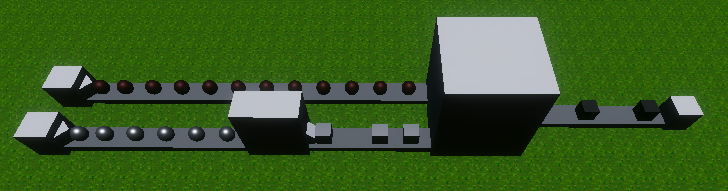
\includegraphics[scale=0.87]{Bilder/Stahl Fabrik.png}
\caption{Eine Stahl Fabrik in der Unity Spielesimulation.}
\label{fig:steel}
\end{figure}
Ganz links befinden sich zwei Kästen. Diese sollen Erzbohrer darstellen welche Eisenerz (silbern) und Kohle (braun) aus der Erde befördern und rechts auf ein Förderband legen. Die beiden Förderbänder transportieren die Kohle und das Eisenerz nach rechts weiter. Das Eisenerz wird als nächstes in Eisenbarren geschmolzen und sind deshalb rechteckig. Die Kohle und die Eisenbarren kommen dann gemeinsam in den großen Würfel, wo sie zu Stahl verarbeitet werden. Dieser Stahl wird dann wieder auf ein Förderband gelegt und in dem kleinen Würfel anschließend gelöscht. Die ganze Produktionskette soll möglichst einem Spiel nahekommen damit es eine möglichst realistische Simulation bietet und die Realität widerspiegelt. Nachfolgend wird gezeigt, wie die Spielsimulation möglichst ähnlich umgesetzt und gebenchmarkt wird.
\subsection{Objektorientierte Programmierung}
In der Objektorientierten Programmierung mit Unity dreht sich alles um GameObjects. Jedes Objekt in der Szene, egal ob sichtbar oder nicht ist ein GameObject. Diese GameObjects können verschiedene Komponenten haben, welche Eigenschaften definieren, also Daten speichern. Diese Komponenten sind jedoch nicht zu verwechseln mit den \textit{Components} aus dem datenorientierten Ansatz von Unity. Diese Komponenten haben jeweils eine \texttt{Start} und eine \texttt{Update} Methode welche das Verhalten definieren. Die Start Methode wird einmalig vor dem ersten Aufruf der \texttt{Update} Methode ausgeführt. Die \texttt{Update} Methode läuft ein mal pro ausgegebenem Bild. Das Skript für das Item sieht wie folgt aus:
\begin{lstlisting}[style=code, caption={Item Komponente OOP}]
using Unity.Mathematics;
using UnityEngine;

public class Item : MonoBehaviour
{
    private int2 pos;
    //Serialisiertes Feld für den Unity Editor
    [SerializeField] private int itemID;

    void Update()
    {
    	//Gegenstand wird zu der übergebenen Position pos bewegt
        transform.position = Vector3.Lerp(transform.position, new Vector3(pos.x, pos.y, -0.5f), Time.deltaTime * 2f);
    }

    public void SetPosition(int2 pos)
    {
        this.pos = pos;
    }

    public int GetItemID()
    {
        return itemID;
    }
}
\end{lstlisting}
Wie man sieht beinhaltet das MonoBehaviour nicht nur die Daten, sondern auch die Logik. Für ein Item benötigen wir zum einen die Position, wohin sich das Item bewegen soll, zum anderen speichern wir auch eine ID über die wir das Item ganz einfach identifizieren können. Das Attribut \glqq SerializeField\grqq{} zwingt Unity dazu ein editierbares Feld im Editor zu erstellen an dem man die itemID setzen kann.
\begin{figure}[H]
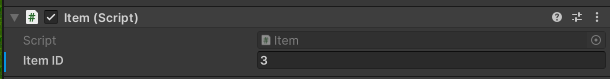
\includegraphics[scale=1]{Bilder/SerializeField.png}
\caption{Ein editierbares Feld in dem Unity Editor. Das Feld wird durch ein public Attribut, oder dem SerializeField Flag erzeugt.}
\label{fig:SerializeField}
\end{figure}
Eine Start Funktion ist in diesem Fall nicht notwendig. Die \texttt{Update} Methode bewegt das Item langsam an die übergebene Position. Time.deltaTime gibt die Zeit in Sekunden von dem letzten Bild bis zu dem momentanen Bild an. Dadurch wird die Bewegung linear.\\Ein weiterer Teil der Simulation ist die Bewegung der Items über das Förderband: 
\begin{lstlisting}[style=code, caption={Förderband Komponente OOP}]
using System.Collections.Generic;
using UnityEngine;

namespace Buildings.Components
{
    public class BeltPath : MonoBehaviour
    {
        private List<ConveyorComponent> beltPath = new ();
        private InputConveyorComponent input;
        private OutputConveyorComponent output;
        private float timeToMove;

        public void Start()
        {
        	//Referenzen auf die Komponenten des GameObjects werden geholt
            input = GetComponent<InputConveyorComponent>();
            output = GetComponent<OutputConveyorComponent>();
            timeToMove = 2f;
        }

        public void Update()
        {
            timeToMove -= Time.deltaTime;
            if(timeToMove > 0) return;
            
            //Gegenstände nach 2 Sekunden bewegen
            var lastBelt = beltPath[^1];
            if (!ReferenceEquals(lastBelt.item, null) && ReferenceEquals(output.GetItem(), null))
            {
            	//Gegenstand von dem letzten Förderbandsegment auf den Output legen
                var item = lastBelt.item;
                var itemComponent = item.GetComponent<Item>();
                itemComponent.SetPosition(output.GetPosition());
                output.SetItem(item);
                lastBelt.item = null;
            }
            //Gegenstände von hinten nach vorne verschieben
            for (int i = beltPath.Count-2; i >= 0; i--)
            {
                var thisConveyor = beltPath[i];
                var lastConveyor = beltPath[i + 1];
                if (!ReferenceEquals(thisConveyor.item, null))
                {
                    if (ReferenceEquals(lastConveyor.item, null))
                    {
                        var item = thisConveyor.item;
                        var itemComponent = item.GetComponent<Item>();
                        lastConveyor.item = item;
                        //Position des Gegenstandes aktualisieren
                        itemComponent.SetPosition(lastConveyor.pos);
                        thisConveyor.item = null;
                    }
                }
            }
            var firstConveyor = beltPath[0];
            //TODO eventuell noch besser machen
            if (!ReferenceEquals(firstConveyor.item, null)) input.SetOccupied(true);
            else input.SetOccupied(false);
            if (!ReferenceEquals(input.GetItem(), null) && ReferenceEquals(firstConveyor.item, null))
            {
                firstConveyor.item = input.GetItem();
                input.RemoveItem();
            }
            timeToMove += 2f;
        }

        public void AddConveyor(ConveyorComponent conveyorComponent)
        {
            beltPath.Add(conveyorComponent);
        }
    }
}
\end{lstlisting}
Für das Förderband wird eine Liste mit vorhandenen Segmenten, der Input, der Output und eine Zeit gespeichert. Die Zeit wird in der Start Methode initialisiert und der Input bzw. Output wird über die Funktion \glqq GetComponent()\grqq{} von dem GameObject geholt. In der \texttt{Update} Funktion wird zunächst nur die timeToMove Variable herunter gezählt. Sollte diese Variable unter Null fallen, werden alle Items von hinten nach vorne ein Segment weiter bewegt sofern dies möglich ist. Ist der Output nicht belegt wird ein vorhandenes Item in den Output gelegt. Items auf den einzelnen Segmenten werden nach weiterbewegt und wenn ein Item im Input liegt wird dies auf das erste Segment weiterbewegt. Immer wenn ein Item weitergegeben wird (egal ob an ein Segment, oder an den Output) wird auch die neue Position an das Item weitergegeben. Durch das bewegen der Items von hinten nach vorne verhindert man, dass sich Items nicht bewegen, obwohl sie es könnten.
\subsection{Datenorientierte Programmierung}
In der datenorientierten Programmierung gehen wir statt der GameObjects auf die Komponenten und Systeme ein. Auch hier zu Beginn die Komponente für ein Item und das dazugehörige System:
\begin{lstlisting}[style=code, caption={Item Komponente ECS}]
using Unity.Entities;
using Unity.Mathematics;

namespace ECS.Components
{
    public struct ItemComponent : IComponentData
    {
        public int2 pos;
        public int itemID;
    }
}
\end{lstlisting}
Auch hier wird die Position und die ID des Items gespeichert. Das dazugehörige System sieht anders aus als das MonoBehaviour im Objektorientierten, die Logik ist jedoch dieselbe:
\begin{lstlisting}[style=code, caption={Item System}]
using ECS.Components;
using Unity.Burst;
using UnityEngine;
using Unity.Entities;
using Unity.Transforms;

[BurstCompile(CompileSynchronously = true)]
public partial struct ItemSystem : ISystem
{
    
    [BurstCompile(CompileSynchronously = true)]
    public void OnUpdate(ref SystemState state)
    {
    	//Job erstellen, Zeit übergeben und schedulen
        new ItemMoveJob
        {
            deltaTime = SystemAPI.Time.DeltaTime
        }.ScheduleParallel();
    }

    [BurstCompile(CompileSynchronously = true)]
    public partial struct ItemMoveJob : IJobEntity
    {
        public float deltaTime;
        
        [BurstCompile(CompileSynchronously = true)]
        private void Execute(ref LocalTransform transform, in ItemComponent item)
        {
        	//Gegenstand wird zu der übergebenen Position pos bewegt
            transform = transform.WithPosition(Vector3.Lerp(transform.Position.xyz, new Vector3(item.pos.x, item.pos.y, -0.5f), deltaTime * 2f));
        }
    }
}
\end{lstlisting}
Jedoch sieht man hier schon Eigenheiten des Entity Component Systems, des Burst Compiler und dem Job System. Das Item System implementiert das Interface ISystem welches für unverwaltete Systeme verwendet werden muss. Zusätzlich ist die Struktur als auch deren Methoden und dem Job mit BurstCompile gekennzeichnet. Diese Kennzeichnung hilft dem Burst Compiler Methoden zu finden, welche mit Burst kompiliert werden sollen. Das Flag CompileSynchronously dient dem testen. Es besagt, dass erst das System durch den Burst Compiler kompiliert werden muss bevor es laufen kann. Andernfalls könnte das System schon laufen, ohne den Burst Compiler genutzt zu haben. Die Methode \texttt{OnUpdate} wird ein mal pro Bild aufgerufen. Sie ist zu vergleichen mit der \texttt{Update} Methode in einem MonoBehaviour. Innerhalb der \texttt{OnUpdate} Methode kommt das Job System von Unity zum Einsatz. Es wird der ItemMoveJob erstellt. Dieser Job funktioniert mit einem LocalTransform Component, welches jedes Entity besitzt und mit dem ItemComponent. Dabei wird das LocalTransform Component zum lesen und schreiben verwendet (erkennbar durch das Keywort ref) und das ItemComponent lediglich zum lesen (erkannbar durch das Keywort in). Auch hier wird nun die Position des Items mithilfe der Lerp Funktion von Vector3 und den Daten im ItemComponent verändert. Dieser Job, welcher die tatsächliche Logik für das Item enthält wird in der \texttt{OnUpdate} Methode parallel gescheduled. Dies ist hier speziell sehr vorteilhaft, da es sehr viele Items auf dem Spielfeld geben kann. Dadurch werden nicht tausende Items nacheinander bewegt, sondern alle zur gleichen Zeit.\\Ein Blick sollte auch auf das Erstellen und Zerstören von Items gelegt werden:
\begin{lstlisting}[style=code, caption={Create Item System}]
using ECS.Components;
using ECS.Components.Other;
using Unity.Burst;
using Unity.Collections;
using Unity.Entities;
using Unity.Mathematics;
using Unity.Transforms;
using UnityEngine;

namespace ECS.Systems
{
    [BurstCompile(CompileSynchronously = true)]
    [UpdateAfter(typeof(ProcessingBuildingSystem))]
    public partial struct CreateItemSystem : ISystem
    {
        private ComponentLookup<InputConveyorComponent> inputLookup;

        [BurstCompile(CompileSynchronously = true)]
        public void OnCreate(ref SystemState state)
        {
        	//Für die OnUpdate Funktion wird das ItemEntitiesComponent gebraucht
            state.RequireForUpdate<ItemEntitiesComponent>();
            inputLookup = state.GetComponentLookup<InputConveyorComponent>();
        }

        [BurstCompile(CompileSynchronously = true)]
        public void OnUpdate(ref SystemState state)
        {
            inputLookup.Update(ref state);
            var ecbSingleton = SystemAPI.GetSingleton<BeginSimulationEntityCommandBufferSystem.Singleton>();
            //Entity Command Buffer wird erstellt
            var ecb = ecbSingleton.CreateCommandBuffer(state.WorldUnmanaged);
            var itemEntities = SystemAPI.GetSingleton<ItemEntitiesComponent>();
            new CreateItemJob
            {
                inputLookup = inputLookup,
                ecb = ecb,
                itemEntities = itemEntities
            }.Schedule();
            state.CompleteDependency();
        }
        
        [BurstCompile(CompileSynchronously = true)]
        [WithNone(typeof(OutputNotFoundTag))]
        public partial struct CreateItemJob : IJobEntity
        {
            public EntityCommandBuffer ecb;
            [ReadOnly] public ComponentLookup<InputConveyorComponent> inputLookup;
            [ReadOnly] public ItemEntitiesComponent itemEntities;

            [BurstCompile(CompileSynchronously = true)]
            private void Execute(ref OutputProcessingBuildingComponent output)
            {
                if(output.itemID == -1) return;
                var itemID = output.itemID;
                var input = inputLookup[output.outputEntity];
                if(input.occupied || input.item != Entity.Null) return;
                output.itemID = -1;
                output.itemCreated = true;
                var itemEntity = itemEntities.GetEntityWithID(itemID);
                var item = ecb.Instantiate(itemEntity);
                ecb.SetComponent(item, LocalTransform.FromPositionRotationScale(new float3(output.pos.x, output.pos.y, -0.5f), quaternion.identity, 0.5f));
                ecb.SetComponent(item, new ItemComponent{pos = output.pos, itemID = itemID});
                ecb.SetComponent(output.outputEntity, new InputConveyorComponent{ item = item, pos = input.pos, occupied = true});
            }
        }
    }
}
\end{lstlisting}
Auch hier sieht man eine Besonderheit des \textit{Entity Component Systems}, der \textit{Entity Command Buffer} (ECB). Dadurch dass strukturelle Änderungen nur auf dem Haupt \textit{Thread} passieren dürfen braucht man einen ECB um diese Änderungen zu sammeln und an späteren Stelle auf dem Haupt \textit{Thread} auszuführem\footnote{https://docs.unity3d.com/Packages/com.unity.entities@1.0/manual/systems-entity-command-buffers.html}. Hier wird der ECB verwendet um strukturelle Änderungen aus einem Job vorzunehmen. Der \textit{Entity Command Buffer} erstellt das Item und ändert noch in den Komponenten die Position des Items.
\newpage
\section{Benchmark}
Um die Benchmark Tests reproduzierbar zu machen gibt es zunächst eine Auflistung der Komponenten, auf denen die Tests durchgeführt wurden: NVIDIA GeForce RTX 3070, Intel Core i7 12700, 32 Gb DDR 4 RAM. Die Tests liefen außerdem auf einem Windows Betriebssystem.\\ In diesem Kapitel wird nun der direkte Vergleich von dem ECS und dem objektorientierten Teil angestellt. Dazu stellt Unity einige hilfreiche Tools zu Verfügung um beispielsweise die Bilder pro Sekunde, in seinem Spiel, zu messen. Auch können man dadurch gut nachvollziehen, wie lange eine Aufgabe, wie zum Beispiel die Ausführung der Update Funktionen, benötigt hat. Bei den nachfolgenden Tests wird jeweils das implementierte Spiel, welches in \hyperref[sec:factory]{Kapitel \ref*{sec:factory}} vorgestellt wurde, verwendet. Es werden immer 2000 Bilder gemessen, wobei die letzten 2000 Bilder aufgezeichnet werden, sobald ein Stahlbarren hinten in dem Kasten angekommen ist (\hyperref[fig:steel]{Abbildung \ref*{fig:steel}}). Zusätzlich werden mehrere Durchläufe gemacht. Angefangen wird mit 100 Fabriken. Diese werden in 100er Schritten erhöht bis zu 1000 Fabriken.
\subsection{Profiler}
Mit dem Profiler kann man in Unity sein Spiel aufzeichnen und Daten über eine festgelegte Anzahl von Bildern sammeln. Dazu gehören die CPU Auslastung, der Speicherverbrauch, wie viel Objekte gezeichnet werden und noch vieles mehr. Während das Spiel läuft gibt werden diese Daten live gezeigt. Zusätzlich lassen sich die Daten auch beim pausieren des Spiel abspeichern und andere Daten laden um sie zu betrachten. Dies sieht man auch in nachfolgender \hyperref[fig:profiler]{Abbildung \ref*{fig:profiler}}. 
\begin{figure}[H]
\centering
\begin{annotatedFigure}
	{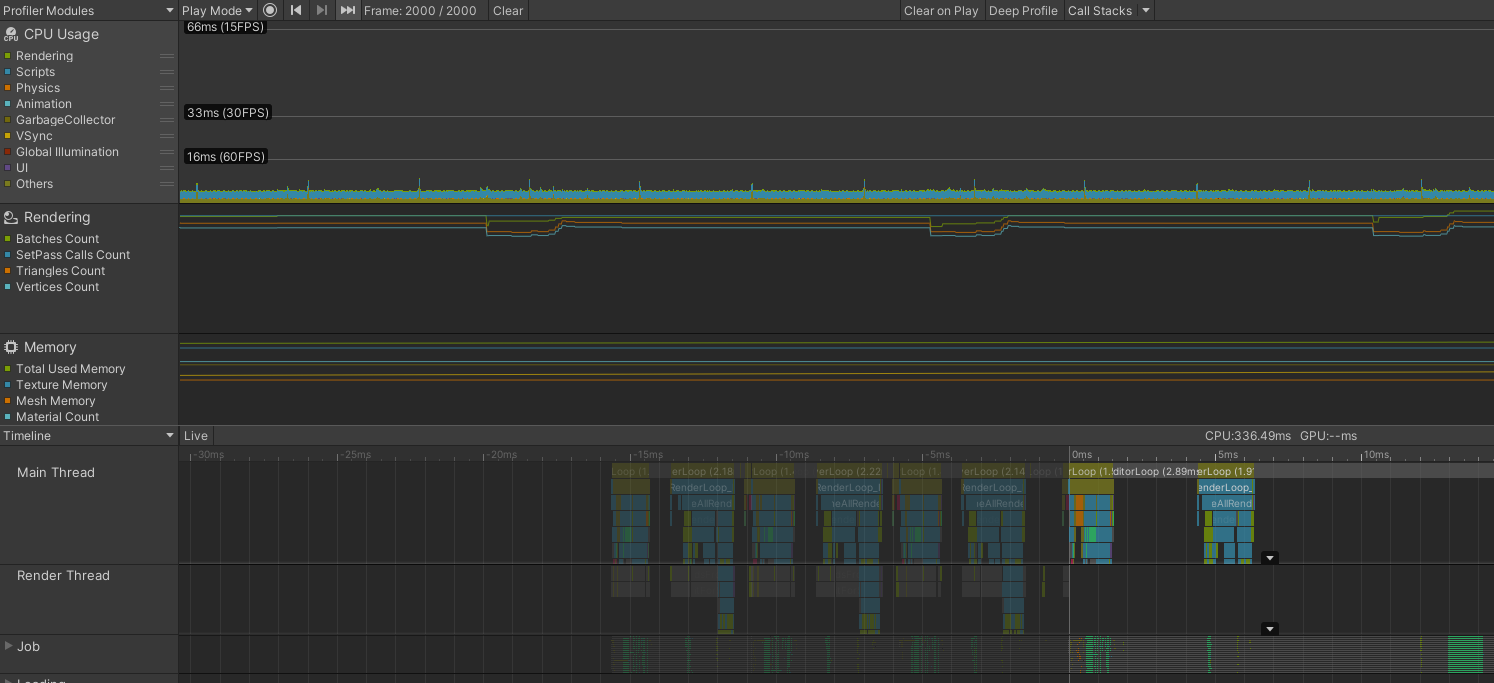
\includegraphics[scale=0.428]{Bilder/Profiler.png}}
    \annotatedFigureBox{0.1688,0.9496}{0.363,1.01}{A}{0.363,0.9496}
	\annotatedFigureBox{0.12,0.65}{1.005,0.76}{B}{1.005,0.65}
	\annotatedFigureBox{-0.005,0.3778}{0.1259,1.01}{C}{0.1259,0.3778}
	\annotatedFigureBox{0.38,0.0888}{0.8705,0.3831}{D}{0.8705,0.0888}
\end{annotatedFigure}
\caption{Der Profiler in dem Unity Editor. Mit ihm lässt sich die Auslastung des Spiels während dem Spielen aufzeichnen und die Daten zur weiteren Verwendung abspeichern. In der oberen Leiste (A), lässt sich das Spiel wie gewünscht aufzeichnen und man sieht die Anzahl an aufgezeichneten Bildern. Man kann auch einzelne Bilder auswählen. Darunter (B) sieht man den Verlauf der aufgezeichneten Bilder. Hier sieht man für jedes Modul eine Auslastung über den Verlauf der 2000 Bildern. Links (C) kann man die einzelnen Module sehen. Sichtbar sind hier die Module CPU Usage, Rendering und Memory, wobei man für weitere im Editor nach unten scrollen muss. Unten (D) ist eine genauere Timeline sichtbar, da hier nur einige Bilder abgebildet werden.}
\label{fig:profiler}
\end{figure}
In dem Bild erkennt man die einzelnen Auslastungen und ihre Kategorien. Zusätzlich kann man ein bestimmtes Bild auswählen und erhält dazu weitere Details in der Timeline weiter unten. Diese aufgezeichneten Daten lassen sich dann in dem Profile Analyzer weiter analysieren.
\subsection{Profile Analyzer}
Der Profile Analyzer dient der weiteren Analyse von aufgenommenen Profilen mit dem Profiler. Zusätzlich hat man mit dem Profile Analyzer die Möglichkeit zwei Profile direkt miteinander zu vergleichen. Dies kann man in \hyperref[fig:profile_analyzer]{Abbildung \ref*{fig:profile_analyzer}} sehen.
\begin{figure}[H]
\centering
\begin{annotatedFigure}
	{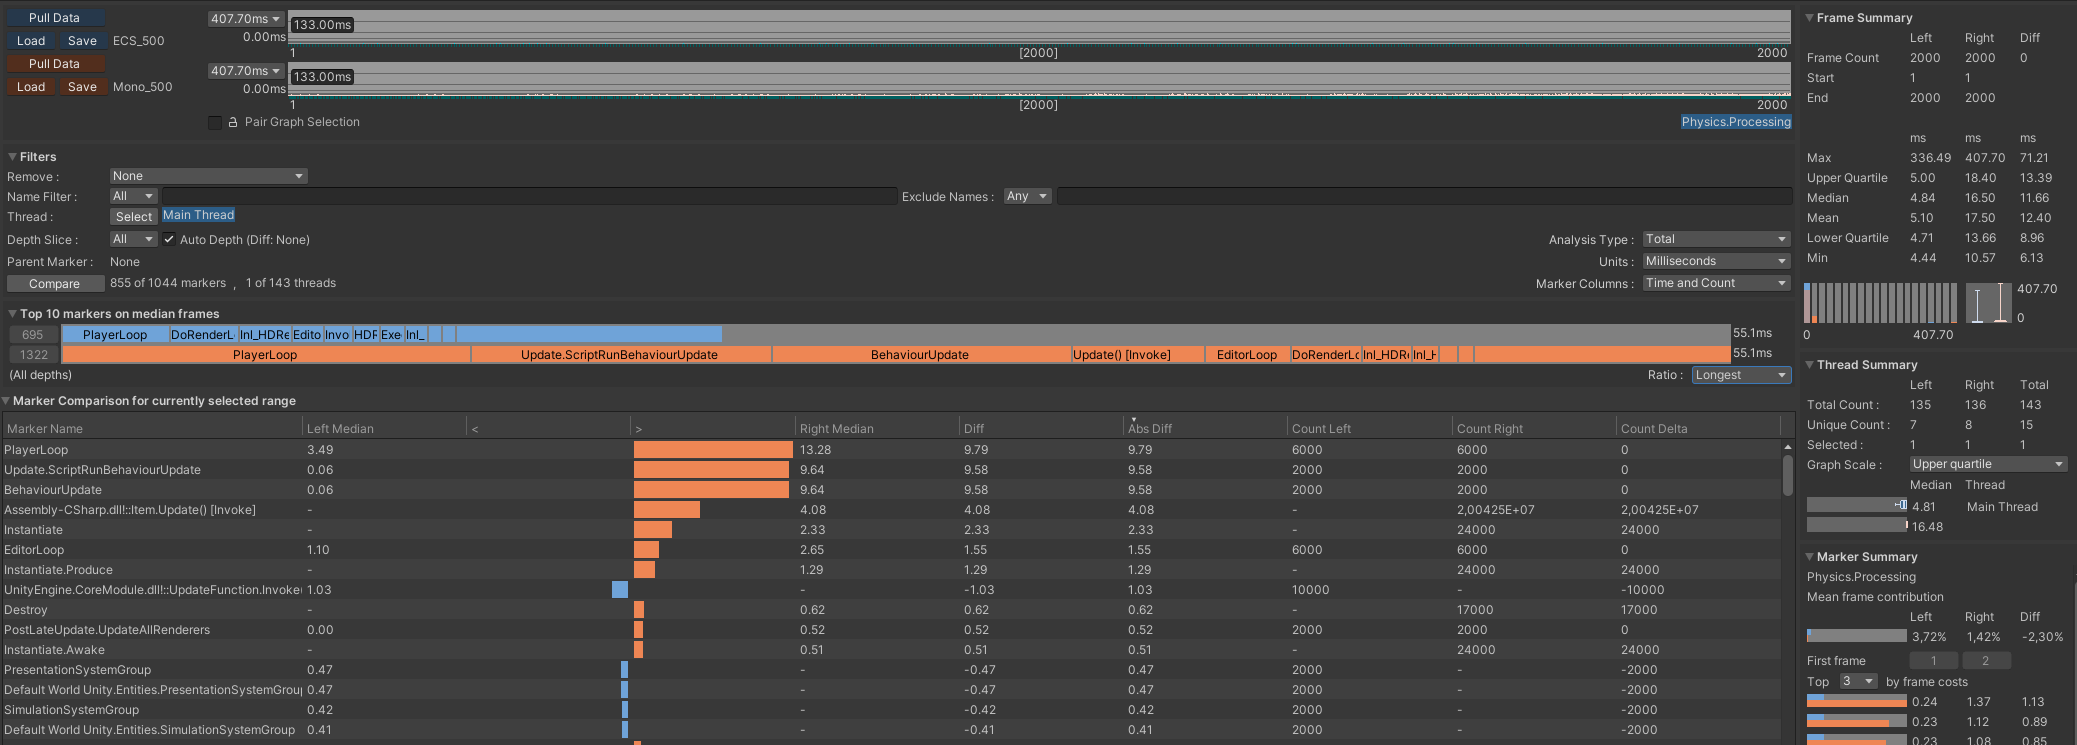
\includegraphics[scale=0.31]{Bilder/Profile Analyzer.png}}
	\annotatedFigureBox{-0.005,0.8046}{0.182,1.01}{A}{0.182,0.8046}
	\annotatedFigureBox{0.86,-0.01}{1.005,1.01}{D}{1.005,-0.01}
	\annotatedFigureBox{-0.005,0.4842}{0.857,0.5942}{B}{0.857,0.4842}
	\annotatedFigureBox{-0.005,-0.01}{0.445,0.4804}{C}{0.445,-0.01}
\end{annotatedFigure}
\caption[Der \textit{Profile Analyzer} im Unity Editor]{Der \textit{Profile Analyzer} im Unity Editor. Es werden die Mono- und die \textit{ECS} Messdaten des Spiels miteinander verglichen. Links oben (A) erkennt man, welche Daten man gerade vergleicht und sieht dazu eine Timeline beider Daten. Die \textit{ECS} Daten sind im Bild blau dargestellt, die Mono Daten rot. In der Mitte des Bildes (B) hat man den Vergleich des Median Bildes. Deutlich zu erkennen ist die wesentlich kürzere Laufzeit des \textit{ECS} Bildes. In dem unteren Teil (C) werden wichtige Spielfunktionen im Vergleich dargestellt. Beispielsweise ist ganz oben der \textit{PlayerLoop} (gesamte Berechnungszeit eines Bildes). Dazu erkennt man an dem Balken, welches der Spiele eine höhere Berechnungszeit hatte. Rechts (D) gibt es zusätzlich noch eine Zusammenfassung über die gesamte Anzahl an Bildern und Threads in beiden Spielen.}
\label{fig:profile_analyzer}
\end{figure}
Oberhalb erkennt man beide Daten die man vergleichen möchte und wie viele Bilder die beiden Daten enthalten. Hier ist erkennbar, dass einmal die Daten von dem ECS mit 500 Fabriken (blau dargestellt) und dem Objektorientierten mit 500 Fabriken (rot dargestellt) verglichen werden. Die wichtigen Teile sind hierbei die zusammenfassende Übersicht (rechts), welche eine Übersicht über alle Bilder oder Threads bietet, und den Vergleich von Kernfunktionen der Spiele, wie beispielsweise der Update Funktionen und dem erstellen, oder zerstören von Objekten. Das Problem hierbei ist jedoch, dass die Kernfunktionen von dem Objektorientierten, anders heißen als die von dem Datenorientierten und man sie somit schlecht gegenüberstellen kann. Würde man zwei Objektorientierte Spiele vergleichen, hätten beide einen PlayerLoop und man würde direkt erkennen, welcher länger gebraucht hat. Dennoch kann man die Zusammenfassung der Bilder gut Nutzen und deshalb werden diese im Folgenden ausgewertet.
\subsection{Vergleich}
\begin{figure}[H]
\centering
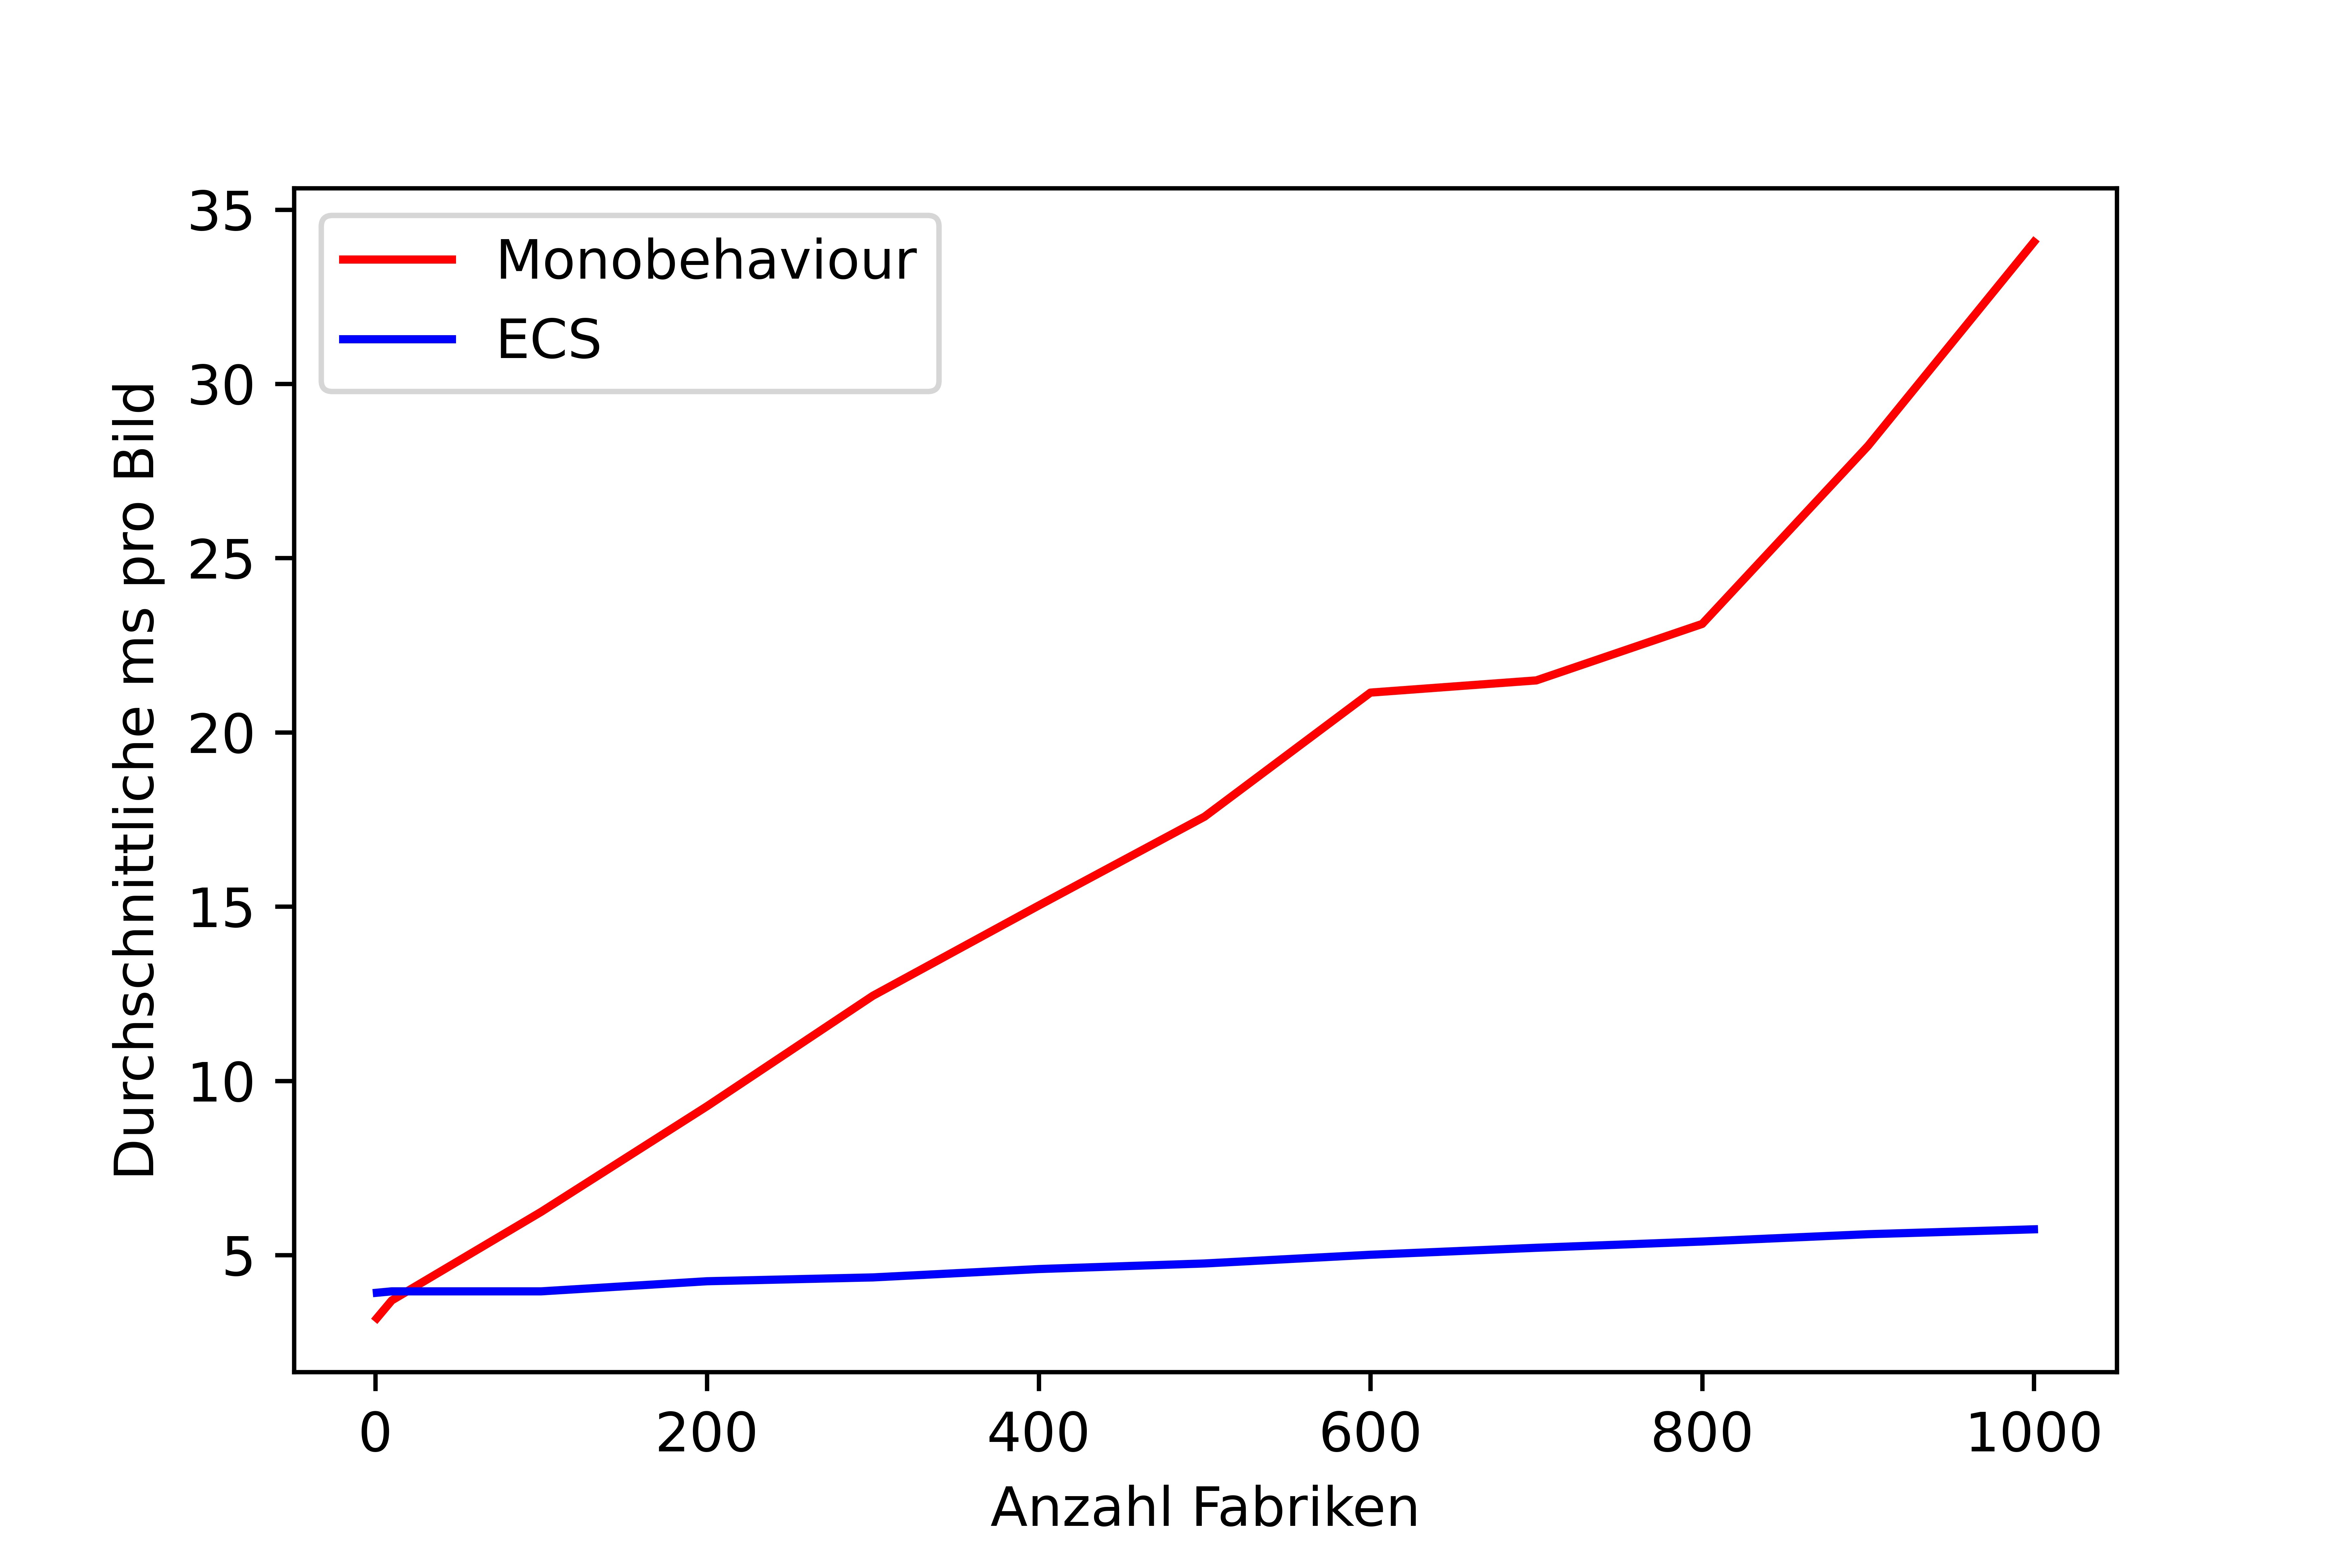
\includegraphics[scale=1]{Bilder/Benchmark.png}
\caption{Der Vergleich von Monobehaviour und dem Entity Component System. Die y-Achse zeigt die durchschnittlichen Millisekunden, die ein Bild gebraucht hat. Die x-Achse zeigt die Anzahl der Fabriken im Spiel.}
\label{fig:benchmark}
\end{figure}
\begin{tabular}[h]{c|c|c}
Anzahl Fabriken & Mittlere Berechnungszeit pro Bild ECS & Mittlere Berechnungszeit pro Bild Mono\\
\hline
100 & 4.3 ms & 6.49 ms\\
200 & 4.48 ms & 10.21 ms\\
300 & 4.73 ms & 12.28 ms\\
400 & 4.91 ms & 15.37 ms\\
500 & 5.1 ms & 17.5 ms\\
600 & 5.32 ms & 19.59 ms\\
700 & 5.52 ms & 21.8 ms\\
800 & 5.72 ms & 24.6 ms\\
900 & 5.92 ms & 25.62 ms\\
1000 & 6.2 ms & 28.61 ms\\
\end{tabular}
\\\\
In \hyperref[fig:benchmark]{Abbildung \ref*{fig:benchmark}} sieht man nun den direkten Vergleich der Laufzeiten von Monobehaviour zu dem ECS. Ganz deutlich erkennbar schneidet das Monobehaviour wesentlich schlechter ab. Das Monobehaviour braucht deutlich länger um ein Bild zu verarbeiten, gerade wenn sich die Anzahl der Fabriken erhöht. Also bestätigt das die Annahme, dass das ECS wesentlich besser darin ist große Mengen an Objekten zu verarbeiten. Auch hier steigt die durchschnittliche Zeit ein Bild zu verarbeiten, jedoch nur sehr gering. 
\newpage
\section{Fazit}
Datenorientierte Programmierung hat großes Potenzial in der Spieleentwicklung. Wie man in der Auswertung gesehen hat ist das \textit{Entity Component System} dem Mono sehr überlegen. Gerade dann, wenn es sehr viele Objekte in der Spielwelt gibt, funktioniert die Verarbeitung der Daten mit einem datenorientierten Ansatz wesentlich schneller. Mit dem Zusammenspiel von Daten und System, welche auf die reine Verarbeitung der Daten spezialisiert sind, kann man außerdem viel Parallelisieren. Dies führt zu einer hohen Effizienz, da der Prozessor besser genutzt wird. Dazu kommt, dass modernere CPU's mehr Kerne haben und diese mit Parallelisierung besser genutzt werden.\\
Jedoch muss man auch betonen, dass das gewählte Beispiel Vorteilhaft für die datenorientierte Programmierung war. Es kommt also auch auf die Anwendung an, ob ein datenorientierter Ansatz einen großen Vorteil bietet. Hat man viel UI, oder ein insgesamt eher kleines Spiel, bringt ein datenorientierter Ansatz nicht viel Performance Optimierung. Auch ist das \textit{Entity Component System} von Unity aufwändig in der Programmierung. Es gibt viel Overhead, vor allem wenn man Objekt zur Laufzeit erstellen möchte. Hier ist jedoch Unity noch in der Entwicklung und wird in Zukunft die Umsetzung des \textit{ECS} einfacher gestalten.\\
Kommt vor allem auf die Anwendung an. Viele gleiche Objekte prima für Datenorientierte Programmierung, da Verarbeitung dann sehr schnell passieren kann. Parallelisierung von Code ist immer gut, neuere CPU's haben immer mehr Kerne, jedoch auch komplexer und man hat zusätzliche Schwierigkeiten. Unity hat momentan noch sehr viel Overhead was die Codegröße betrifft, wird sich mit der Zeit aber auch noch ändern. Schwierig zu entscheiden wird es bei Projekten mit sehr viel UI / wenig gleichen Objekten.
\newpage 
\thispagestyle{empty}
\quad
\newpage
\lstlistoflistings
\newpage
\listoffigures
\newpage
\section{Literaturverzeichnis}
\bibliographystyle{plain}
\bibliography{bibliography}

\newpage
\section{Anlagen}
\newpage
\thispagestyle{empty}
\section*{Selbstständigkeitserklärung}
Ich, Dennis Untiet, erkläre, dass ich die vorliegende Arbeit selbstständig und nur unter Verwendung der
angegebenen Quellen und Hilfsmittel angefertigt habe.\\
Seitens des Verfassers bestehen Einwände die vorliegende Bachelorarbeit für die öffentliche Benutzung im
Universitätsarchiv zur Verfügung zu stellen.\\
Jena, \today, Unterschrift des Verfassenden
\end{document}
